\documentclass[twocolumn]{revtex4-2}

\usepackage{graphicx}

\begin{document}
\title{Water Electrolysis}
\author{Sixten Nordegren}

\date{\today}

\maketitle
\section{Introduction}
Here is a section introducing the rest of the document.
\section{Method}
Three electrodes where lowered down into water with the electrolyte mixed into it.
One Working Electorde (\textbf{We}) from which all the measurments are made. One counter
electrode (\textbf{Ce}) that was placed in the water in order to esablish a 
homogenous electric field. And lastly a final measuring electrode were inserted
into the mixture in order to make proper measurments of the wokring electorde.

On the end of the \textbf{We} and the \textbf{Ce} two metals are attatched acting 
as catalysts for the chemical reaction. 

Current was sent thorught the working electrode via a current generator. Increased
from zero to a set value and working down to that same set value but with changed 
polarity.

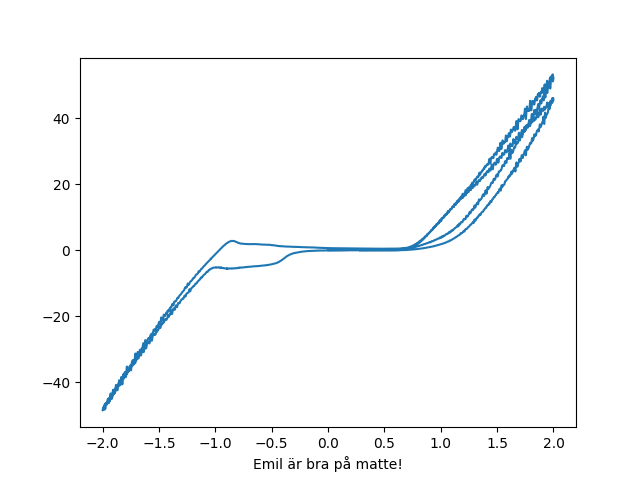
\includegraphics[widht=0.9\linewidth]{/home/sixten/water_electorlysis/data_analysis/data_plot_0.png}
\end{document}

